\documentclass[aspectratio=169]{beamer}
\usepackage{spc}
\begin{document}

\begin{frame}
  \title{\darkblue 2 ~ Git Commands and User Interface}
  \author{\darkgray\bf Arni Magnusson\\
    \phantom{.}\h{32ex}
\includegraphics[width=1cm]{github_logo}}
  \date{\darkgreen SPC Git/GitHub Workshop\\[0.5ex]
    Noumea, 13 April 2022}
  \titlepage
\end{frame}

% ______________________________________________________________________________

\begin{frame}{Overview}
  \begin{itemize}
    \item[] \hyperlink{first}{\bf\darkblue First steps}
    \comment{clone, status, diff}\\[4ex]
    \item[] \hyperlink{submit}{\bf\darkblue Submitting changes} \comment{add,
      commit, push}\\[4ex]
    \item[] \hyperlink{refresh}{\bf\darkblue Refresh and document}
    \comment{pull, log, tag}\\[4ex]
    \item[] \hyperlink{undo}{\bf\darkblue Undo things} \comment{rm, checkout,
      clean, reset}\\[4ex]
    \item[] \hyperlink{ui}{\bf\darkblue User interface}
    \comment{command line, rstudio, web browser, other}\\[1ex]
  \end{itemize}
\end{frame}

% ______________________________________________________________________________

\begin{frame}\Large
  \hypertarget{first}
  \centering\darkgreen\bf
  First Steps
\end{frame}
% ______________________________________________________________________________

\begin{frame}{First Steps}\small
  \vspace{4ex}
  \begin{description}
    \item[\bf clone] Download a copy of remote repo to your computer\\[6ex]
    \item[\bf status] See files you have changed\\[6ex]
    \item[\bf diff] See lines you have changed\\[10ex]
  \end{description}
  \darkblue\it\fns .git is a hidden folder containing a database of tracked
  changes
\end{frame}

% ______________________________________________________________________________

\begin{frame}\Large
  \hypertarget{submit}
  \centering\darkgreen\bf
  Submitting Changes
\end{frame}
% ______________________________________________________________________________

\begin{frame}{Submitting Changes}\small
  \vspace{4ex}
  \begin{description}
    \item[\bf add] Specify files to commit\\[6ex]
    \item[\bf commit] Describe what was changed\\[6ex]
    \item[\bf push] Upload to remote repo\\[10ex]
  \end{description}
  \darkblue\it\fns 3-step combo move
\end{frame}

% ______________________________________________________________________________

\begin{frame}{Submitting Changes}\small
  \vspace{4ex}
  \begin{tabular}{ccccc}
    \darkgreen add
    && \darkgreen commit
    && \darkgreen push\\[1.5ex]
    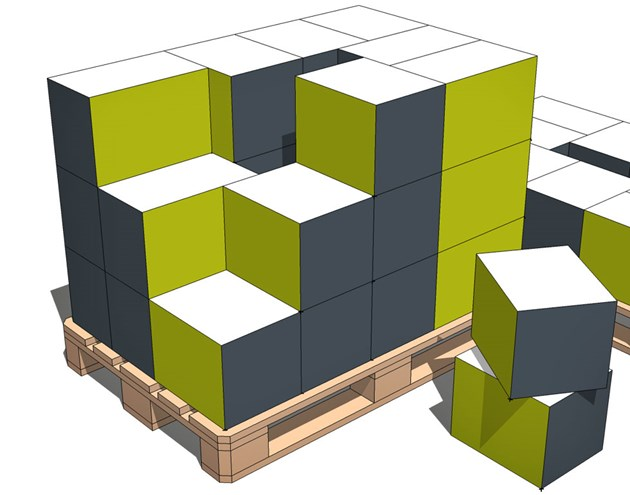
\includegraphics[height=0.3\textheight]{add}
    & ~~\raisebox{8ex}{$\rightarrow$}~~
    & 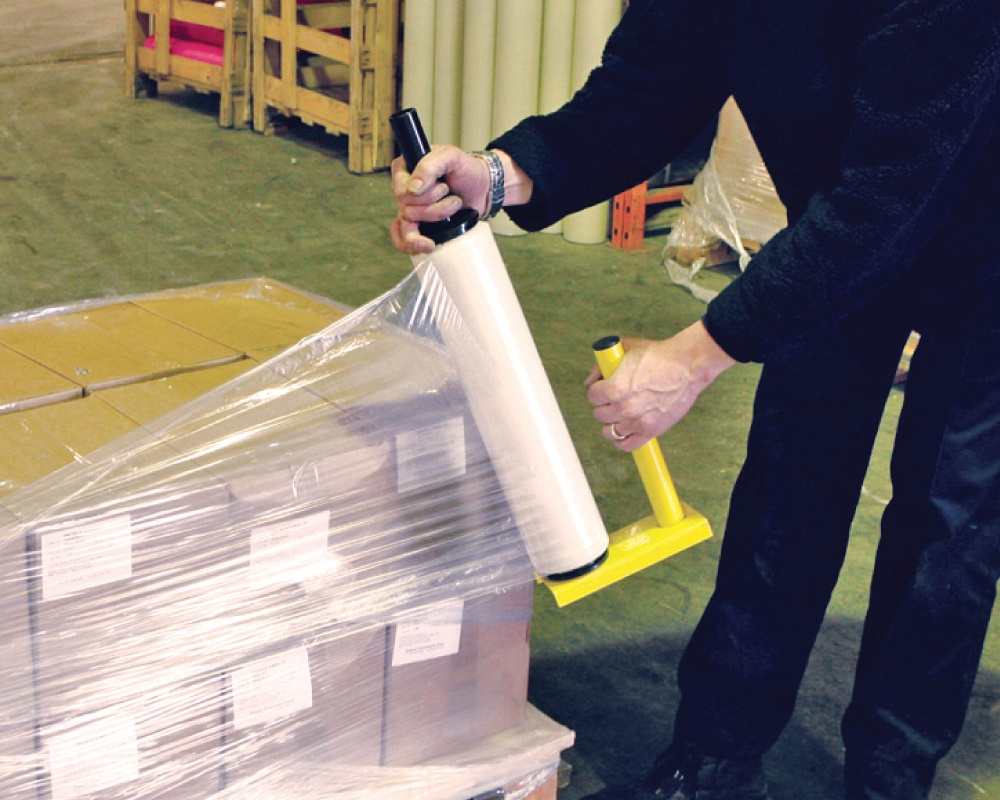
\includegraphics[height=0.3\textheight]{commit}
    & ~~\raisebox{8ex}{$\rightarrow$}~~
    & 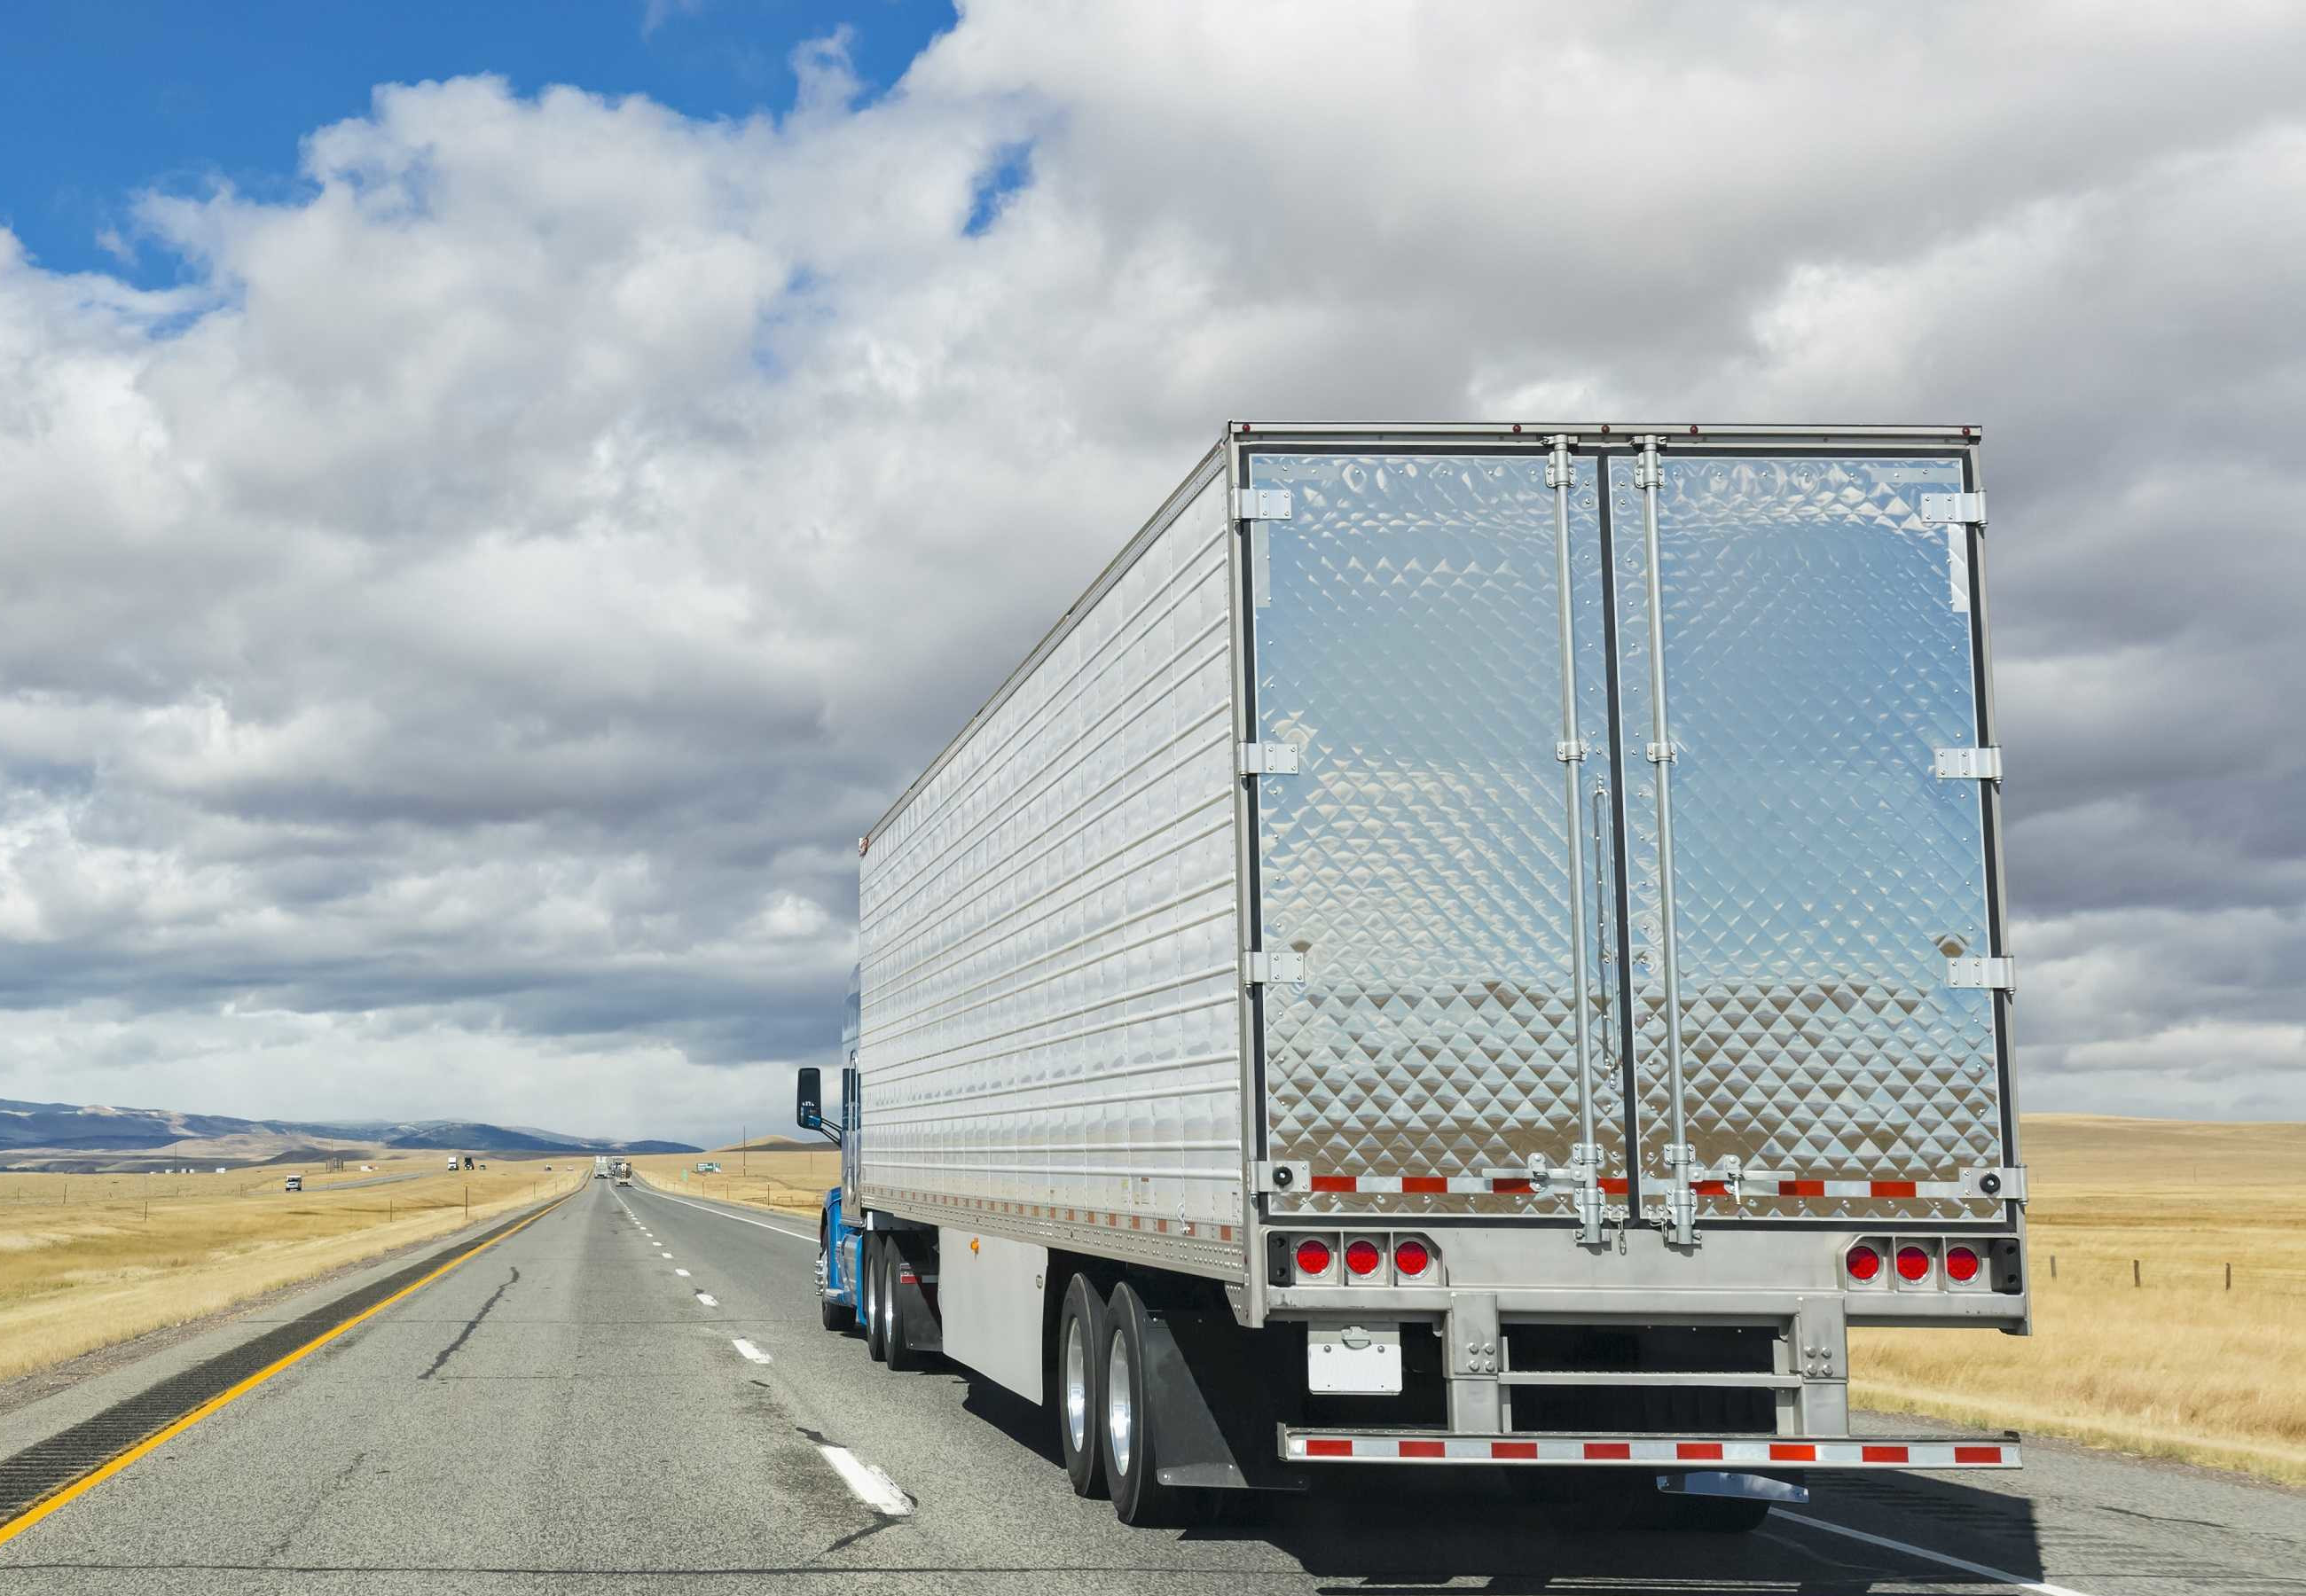
\includegraphics[height=0.3\textheight]{push}\\[2ex]
    select boxes && wrap and label && send it off\\
    that go together
  \end{tabular}
\end{frame}

% ______________________________________________________________________________

\begin{frame}{Commit Messages}\small
  {\bf\darkgray Tips for writing commit messages}
  \begin{itemize}
    \item[] Relatively short \comment{$\sim60$ char}
    \item[] Describe purpose \comment{or specific things that were changed}
    \item[] Present tense \comment{often starting with a verb like `Add',
      `Improve', `Document', ...}
  \end{itemize}
  \vspace{3ex}
  {\bf\darkgray Examples}
  \begin{itemize}\blue
    \item[] \href{https://github.com/PacificCommunity/ofp-sam-mfcl/commits}
    {MFCL}
    \item[] \href{https://github.com/PacificCommunity/ofp-sam-skj22/commits}
    {skj22}
    \item[] \href{https://github.com/PacificCommunity/ofp-sam-yft-2017/commits}
    {yft-2017}
  \end{itemize}
\end{frame}

% ______________________________________________________________________________

\begin{frame}{Commit Messages}\small
  \centering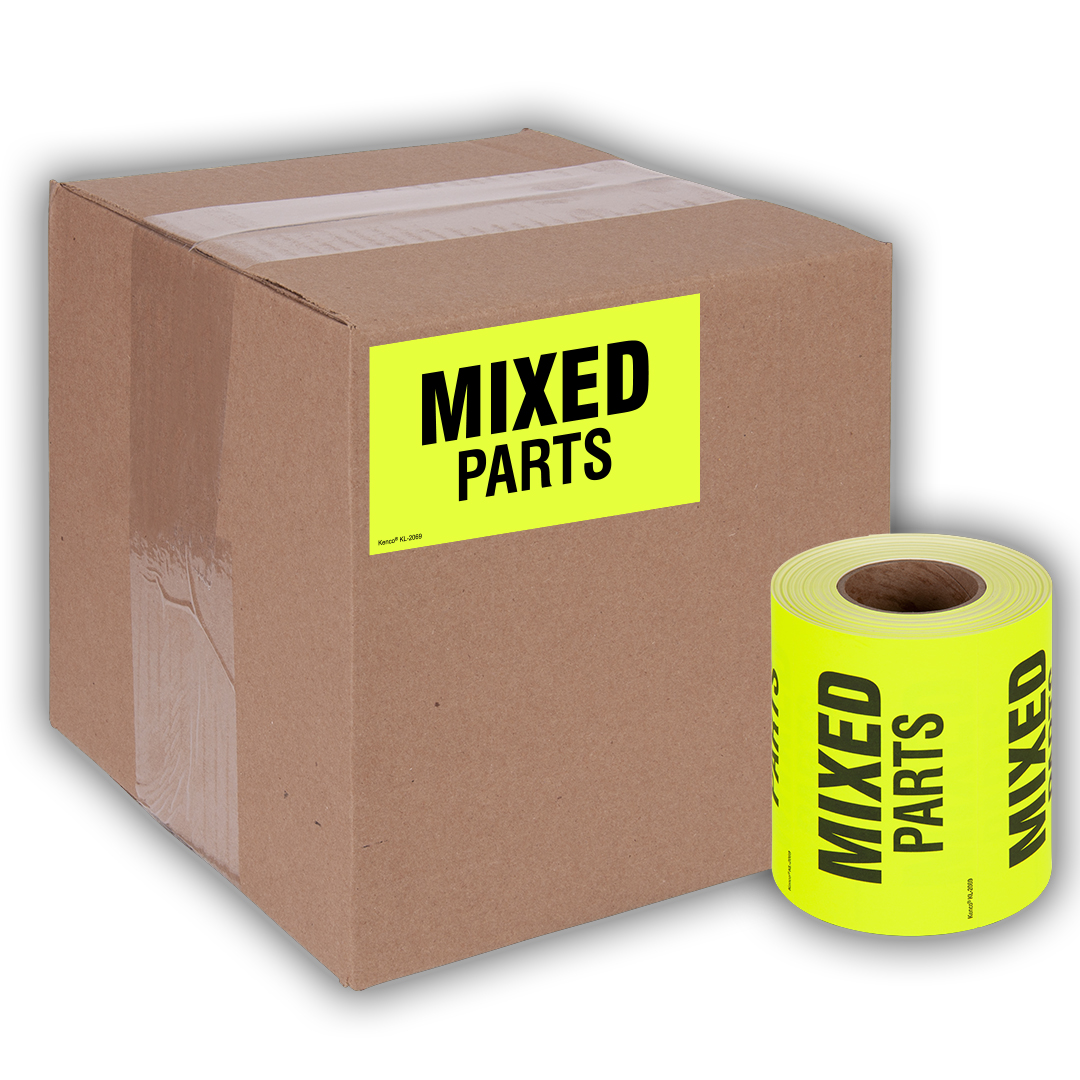
\includegraphics[height=0.5\textheight]{message}
\end{frame}

% ______________________________________________________________________________

\begin{frame}\Large
  \hypertarget{refresh}
  \centering\darkgreen\bf
  Refresh and Document
\end{frame}

% ______________________________________________________________________________

\begin{frame}{Refresh and Document}\small
  \begin{description}
    \item[\bf pull] Refresh local repo \comment{download latest commits from
      remote repo}\\[6ex]
    \item[\bf log] View commit messages \comment{can also view on
      github.com}\\[6ex]
    \item[\bf tag] Mark significant commit with a nickname \comment{example:
      2.0.0}\\[2ex]
  \end{description}
\end{frame}

% ______________________________________________________________________________

\begin{frame}\Large
  \hypertarget{undo}
  \centering\darkgreen\bf
  Undoing Things
\end{frame}

% ______________________________________________________________________________

\begin{frame}{Undoing Things}\small
  \begin{description}
    \item[\bf rm] Remove file from repo \comment{it will still be `remembered'
      in history}\\[5ex]
    \item[\bf checkout] Undo local changes
    \comment{\fns\tt git checkout -- file}\\[1.5ex]
    (also) Select branch\\[5ex]
    \item[\bf clean] Remove files that are not part of the repo
    \comment{example: MFCL output files}\\[5ex]
    \item[\bf reset] Rewind to a previous snapshot of the project \comment{pull
      to go back to the `present'}\\[1.5ex]
    (also) Un-add files\\
  \end{description}
\end{frame}

% ______________________________________________________________________________

\begin{frame}\Large
  \hypertarget{ui}
  \centering\darkgreen\bf
  User Interface
\end{frame}

% ______________________________________________________________________________

\begin{frame}{User Interface}\small
  \begin{description}
    \item[\bf Command line] Works on all computers, full Git
    functionality\\[0.8ex]
    \h{-0.1ex}\comment{especially practical if you know the basic shell
      commands}\\[5ex]
    \item[\bf RStudio] Convenient if you're already using RStudio\\[0.8ex]
    \h{-2ex}\comment{small subset of Git commands, noticeable lag, creates
      `garbage' files}\\[5ex]
    \item[\bf Web browser] Commit history, files and lines changed, GitHub
    features\\[5ex]
    \item[\bf Other] Most editors have Git support, also many dedicated Git
    clients\\[0.8ex]
    \h{-2.1ex}\comment{view current changes (not yet committed)}
  \end{description}
\end{frame}

% ______________________________________________________________________________

\begin{frame}{User Interface (cont)}\small
  Arni's shell {\blue\href{https://github.com/arni-magnusson/bin}{scripts}} and
  {\blue
    \href{https://github.com/arni-magnusson/dot/blob/master/.bashrc}{aliases}}
  \begin{itemize}\fns
    \item[] add, br, clone, co, commit, di, log, merge, pull, push, reset, show,
    st, stash, tag \comment{\fns shorthand}
    \item[] c \comment{\fns clone and rename OFP-SAM repo}
    \item[] commits \comment{\fns that are not yet pushed}
    \item[] eg \comment{\fns Emacs Magit}
    \item[] files \comment{\fns that were changed in a given commit}
    \item[] lfh \comment{\fns\tt log-full | head}
    \item[] shortlog \comment{\fns show commits by author}
    \item[] tag-delete \comment{\fns remote repo}
    \item[] url \comment{\fns show remote repo location}
    \item[] br-full, commits-full, files-full, log-full, shortlog-full,
    show-full, tag-full
  \end{itemize}
\end{frame}

% ______________________________________________________________________________

\begin{frame}{Summary}
  \begin{itemize}
    \item[] \hyperlink{first}{\bf\darkblue First steps}
    \comment{clone, status, diff}\\[4ex]
    \item[] \hyperlink{submit}{\bf\darkblue Submitting changes} \comment{add,
      commit, push}\\[4ex]
    \item[] \hyperlink{refresh}{\bf\darkblue Refresh and document}
    \comment{pull, log, tag}\\[4ex]
    \item[] \hyperlink{undo}{\bf\darkblue Undo things} \comment{rm, checkout,
      clean, reset}\\[4ex]
    \item[] \hyperlink{ui}{\bf\darkblue User interface}
    \comment{command line, rstudio, web browser, other}\\[1ex]
  \end{itemize}
\end{frame}

\end{document}
